\documentclass[11pt]{article}
\usepackage[utf8]{inputenc}
\usepackage{amsmath, amssymb}
\usepackage{graphicx}
\usepackage{hyperref}
\usepackage{geometry}
\usepackage[backend=biber]{biblatex}
\addbibresource{../references.bib}
\geometry{margin=1in}

\title{The Abstract Universe Project: Technical Introduction}
\author{Abstract Author}
\date{\today}

\begin{document}

\maketitle

\section{Introduction}

This paper presents the foundational assumptions and conclusions that lead to \href{run:./paper2.pdf}{the Abstract Universe Project}  — a radically minimalistic approach to a theory of everything, grounded purely in information theory. The core idea is that all physical reality, including conscious observers, spacetime, and matter, can be derived from finite set of compressed information. By applying principles of computational theory and observer-centric reasoning, the theory posits that familiar physics — including gravity and quantum mechanics — emerges pure abstract information. The observer, rather than being external, is modeled as a subset within a finite universe, offering a self-contained, emergent, and minimal framework of physics.


\section{Philosophical Elegance — Mathematical Minimalism}

This is a theory of physics. The only philosophical principle introduced is the requirement that the theory be free of any predefined substrate. It must be self-contained, with all physical laws arising as emergent properties rather than as assumed primitives.

From this perspective, we critique existing physical theories. As an example, Standard Model of quantum mechanics depends on at least 19 empirical constants, whose values are not derived within the theory.

The Abstract Universe Project starts with four physically reasonable observational assumptions \href{run:./paper2.pdf}{Physics as an Emergent Property of the Observer: A Derivation from Four Assumptions}. The rest is what follows.



\section{The Observational Assumptions}

\begin{itemize}
      \item \textbf{Assumption 1:} DNA Contains Sufficient Information for building conscious observer.
      \item \textbf{Assumption 2:} DNA consists of ordinary matter, and therefore obeys Physical Laws.
      \item \textbf{Assumption 3:} The Church–Turing Thesis Holds, stating that all physical laws can be duplicated using Turing Machine (computer)
      \item \textbf{Assumption 4:} Pain Has Measurable Physical Effects.
\end{itemize}

The fourth assumption:

\[
      \text{Human} + \text{Pain} \neq \text{Human}
\]

is essential for bringing consciousness out of the realm of purely philosophical or subjective discourse and into the domain of physics.

If a human experiencing pain behaves differently from one who does not, then pain produces measurable effects, allowing for the falsification of this theory's predictions. This reasoning extends to other subjective experiences.

% ------

\section{Information}

We do not fully understand what information is at its core. Similarly, the fundamental nature of human consciousness remains elusive.  However, assuming the four observational assumptions hold, everything within human consciousness can, in principle, be duplicated using a Turing machine or its modern counterpart—a computer. From this, we derive:

\begin{itemize}
      \item Computers are based on binary systems, whose operations are formally understood, and
      \item Set theory is sufficient to describe the structure of binary computation,
\end{itemize}

Therefore binary systems—bits—are a sufficient and complete informational foundation to describe reality.

Since set-theoretical descriptions can be lengthy, we use the term "bitstring" as a synonym for an ordered set of binary elements.


\section{Definition of Reality}

What we perceive as reality is not an exact substrate; it appears to consist of matter particles (fermions), which we can measure and therefore consider real. However, the same mathematical descriptions also predict virtual particles (bosons), which we cannot directly measure and therefore do not regard as real.

We define reality as the set of observable phenomena that can, in principle, be measured and whose outcomes can be compared to predictions made by the theory. This definition aligns with the scientific method.


% ------



\section{Universe with Observer in It}

We start by defining observations that the theory must be able to predict:

We observe a vast universe \( U \) that includes ourselves as tiny subsets. To model this, we define:

\[
      O \subseteq U
\]

We also observe time as a unidirectional flow, advancing continuously and carrying us through the evolving universe:

\[
      \forall t_1, t_2 \in T,\quad t_2 > t_1 \Rightarrow t_2 \text{ is in the future of } t_1
\]

We observe an universe in which information cannot be created or destroyed, only transformed.

\[
      I(t_1) = I(t_2) \quad \forall \, t_1, t_2
\]

Where I(t)I(t) is the information content of a closed system at time t. This expresses the idea that information is invariant under time evolution—a principle respected by unitary evolution in quantum mechanics.



% ---------


\section{The Abstract Universe Project}

We use bits as the elementary building blocks of the universe. The universe \(U\) is modeled as a finite bitstring. The observer \(O\) is modeled as a substring within \(U\).

As shown in \cite{meskanen2019}, a bitstring of pure noise, given sufficient length, will eventually describe a conscious observer. The information in \(n\) bits can be arranged in \(2^n\) ways.

Let \(O \subseteq U\) be an observer embedded within the universe. Suppose the internal informational state of the observer is encoded by a bitstring of length \(n\). Then the number of possible configurations is:

\[
      |\mathcal{C}| = 2^n
\]

Let \(\mathcal{C}_{\text{conscious}} \subseteq \mathcal{C}\) be the subset corresponding to coherent, intelligent, and conscious observers. Then the probability of consciousness is:

\[
      P_{\text{conscious}} = \frac{|\mathcal{C}_{\text{conscious}}|}{2^n}
\]

This quantifies how rare or typical conscious arrangements are within the space of all informational configurations.

From a purely statistical standpoint, the likelihood of a universe with parameters finely tuned for the emergence of us appears vanishingly small.

This could be understood through an anthropic or observer-selection principle: only those configurations of the universe that allow for observers can be observed, rendering our presence a conditional inevitability rather than an improbability.

The explanation does not, by itself, qualify as a physical theory. It is incapable to make predictions.


\subsection{The Problem with Memory}

A viable theory must account for the emergence of observers with memory, capable of acquiring and retaining information about their environment.

For an observer to remember or perceive anything, their bitstring must contain information reflecting the external universe. 
How can information be transmitted from the superstring representing the universe to the substring representing the observer? 

Since the system is entirely self-contained, no external signals can transmit information; thus, within the framework of set theory, 
any knowledge the observer possesses must already be embedded in their bitstring.

\begin{figure}[h!]
      \centering
      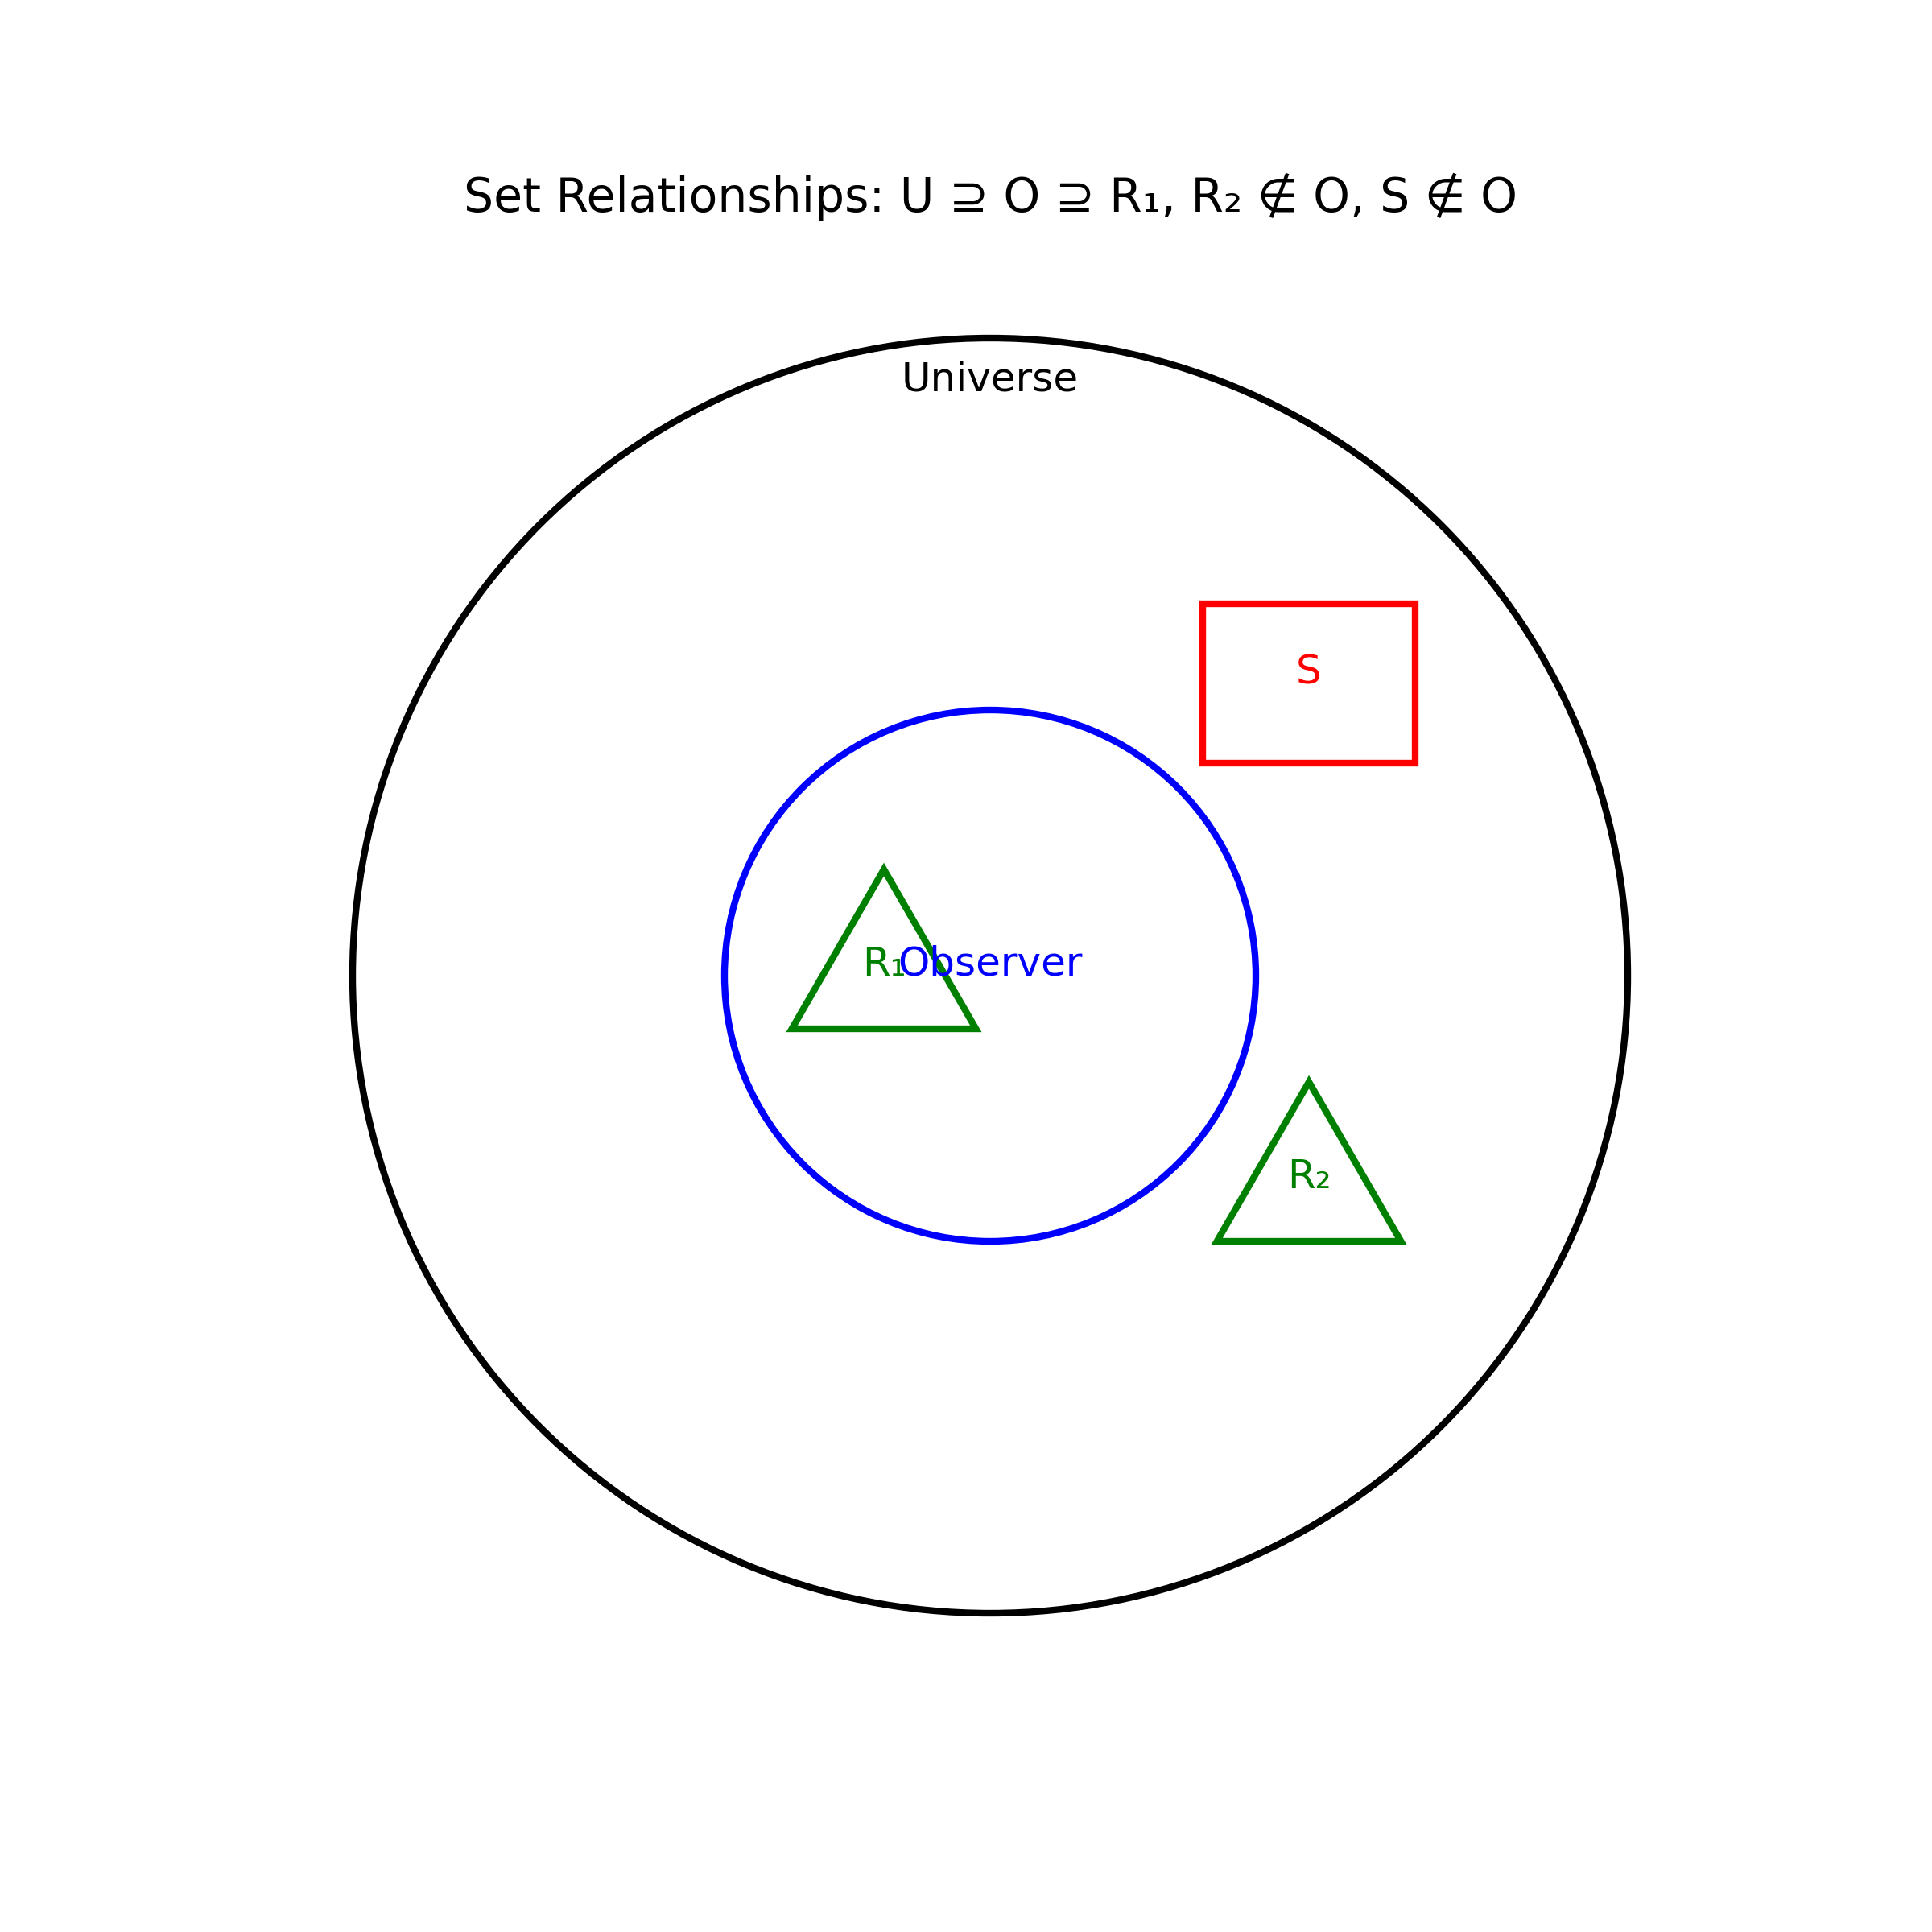
\includegraphics[width=0.6\textwidth]{figures/memory.png}
      \caption{An observer with embedded knowledge about the surrounding universe ($R_1$). (S) represents information not included within the observer.}

      \label{fig:memory}
\end{figure}

\textbf{Conclusion:} Observers are most likely to find themselves in bitstrings that describe both the observer and the 
surrounding observable universe.



\subsection{The Nature of the Wavefunction}

The observer-centric principle naturally explains the apparent randomness of reality: rather than being defined by a single exact bitstring, observers can exist across multiple bitstrings—those that describe them with sufficient precision—thereby increasing the probability of their existence. But what accounts for the wave-like nature of the universe?

The wavefunction is deterministic and defines probabilistic outcomes. We argue this duality has a logical basis.

\subsection{The Wavefunction as a Compression Algorithm}

From two assumptions:

\begin{itemize}
      \item The observer-centric principle: the observer can only find themselves from universes that describe them.
      \item Universes that describe more observers are more probable.
\end{itemize}

we conclude that the wavefunction is a compression algorithm.

\textbf{Conclusion:} The wavefunction is a compression algorithm for describing a conscious observer using a minimal number of bits. The sine wave, being the simplest periodic function, emerges naturally and leads to quantum mechanics.



\subsection{The Wavefunction Smoothness Problem}

In traditional quantum mechanics, the wavefunction is continuous, implying that it cannot be represented using a finite set of bits.

This raises a dilemma: either our current understanding is incomplete, or the wavefunction is not truly infinitely smooth.

Empirically, we observe that the universe follows a principle of economy—it expresses everything using the minimal possible resources.

Therefore we propose that the wavefunction is, in fact, a discrete structure that only appears smooth due to the universe’s large informational content.

This leads to a theory that better explains our existence by describing us as a compressed set of information, thereby increasing the likelihood of our existence.


\subsection{Observer Compressed}

As the theory must be self-contained, we reject external compression mechanism. \textbf{Oserver's} bitstring must encode descriptions of both data and compression algorithm. We define \textbf{Observer} as the result of an algorithm applied to a wavefunction:

\begin{equation}
      \text{Observer} = A(\Psi)
\end{equation}

where:
\begin{itemize}
      \item \( \Psi \) is the wavefunction representing the observer's quantum state (frequencies, phases),
      \item \( A \) is the algorithm (e.g., Schrödinger dynamics) that evolves or evaluates the wavefunction.
\end{itemize}

\vspace{1em}


\textbf{Conclusion}: The observer bitstring is the wavefunction.


%  ---------

\section{Subjective Time and Wavefunction Evolution}

As derived from the four assumptions \cite{meskanen2019} time must be a intrinsic property of observer. This rises the question how time can emerge natively in observer's wave function?

\subsection*{The Observer Inside a Pure-State Universe}

Following Everett \cite{everett1957relative}, Hartle and Hawking \cite{hartle1983wave}, and others \cite{maldacena1998largeN, witten1998ads, rovelli1997loop}, we model the universe as a pure wavefunction \(|\Psi\rangle\) in Hilbert space \(\mathcal{H}_U\).

We define:

\[
      \mathcal{H}_U = \mathcal{H}_O \otimes \mathcal{H}_R
\]

where:
\begin{itemize}
      \item \(\mathcal{H}_U\) is the Hilbert space of the entire Universe,
      \item \(\mathcal{H}_O\) is the Hilbert space corresponding to the observer subsystem,
      \item \(\mathcal{H}_R\) is the Hilbert space of the rest of the Universe (i.e., all degrees of freedom external to the observer),
      \item and \(\otimes\) denotes the tensor product, indicating that the total Hilbert space is composed of the observer and the rest as subsystems.
\end{itemize}


The observer's reduced state is:

\[
      \rho_O = \mathrm{Tr}_R \left( |\Psi\rangle \langle \Psi| \right)
\]


where:
\begin{itemize}
      \item \(|\Psi\rangle\) is the pure state of the entire Universe in the total Hilbert space \(\mathcal{H}_U = \mathcal{H}_O \otimes \mathcal{H}_R\),
      \item \(\rho_O\) is the **reduced density matrix** of the observer,
      \item \(\mathrm{Tr}_R\) denotes the **partial trace** over the degrees of freedom in \(\mathcal{H}_R\), the Hilbert space of the rest of the Universe.
\end{itemize}

This operation effectively "traces out" the environment (everything other than the observer), yielding the observer's local quantum state.

If the universal state \( |\Psi\rangle \) is \textbf{entangled} between the observer and the rest of the Universe, then \( \rho_O \) will be a \textbf{mixed state} (i.e., not pure). This reflects the fact that the observer is correlated with external degrees of freedom and cannot be described by a pure state alone.

We propose that this gives rise to the observer's sense of time. If the observer were described by a pure-state wavefunction, they would know everything ``now.'' However, being a \textbf{subset} of the universe introduces a self-referential problem, where the observer is forced to describe the universe as an ensemble of \textbf{impure states}, which are numerous.

The illusion of time is a natural result of the observer’s internal state evolving from one bitstring configuration to the next.


\subsection*{Time as Ensemble Indexing}

We define time as a sequence of informational states:

\[
      T = \{ \psi_0, \psi_1, \psi_2, \ldots \}
\]

Each \(\psi_t\) encodes the observer’s state at time \(t\).

\subsection*{Unitary Evolution}

Evolution is modeled as:

\[
      \psi_{t+1} = O \psi_t
\]

where \(O\) preserves continuity and maximizes internal compressibility.


\section{Compression and Emergent Physics}

Smooth and continuous configurations compress better than irregular and non-continuous. To maximize the probability of existence, configurations with minimal algorithmic complexity are therefore favoured.

\[
      \min_O C(O)
\]

It is likely that observers will find themselves in universes that are smooth and continuous—worlds that follow predictable laws of physics.

\printbibliography

\end{document}
